% BreezeSwap Whitepaper
% Build: tectonic breezeswap-whitepaper.tex
\documentclass[11pt,a4paper]{article}

\usepackage[T1]{fontenc}
% amsmath/amssymb must precede newtxmath, which redefines \Bbbk otherwise.
\usepackage{amsmath,amssymb}
\usepackage{newtxtext,newtxmath}
\usepackage[margin=2.6cm,top=2.9cm,bottom=2.9cm]{geometry}
\usepackage{booktabs}
\usepackage{array}
\usepackage{tabularx}
\usepackage{longtable}
\usepackage{xcolor}
\usepackage{tikz}
\usepackage{pgfplots}
\usepackage{caption}
\usepackage{subcaption}
\usepackage{microtype}
\usepackage{titlesec}
\usepackage{fancyhdr}
\usepackage{enumitem}
\usepackage{url}
\usepackage[hidelinks,breaklinks]{hyperref}

\usetikzlibrary{arrows.meta,positioning,fit,backgrounds,calc,shapes.geometric}
\pgfplotsset{compat=1.18}

% ------------------------------------------------------------------
% Palette
% ------------------------------------------------------------------
\definecolor{bzblue}{HTML}{1F4E79}
\definecolor{bzteal}{HTML}{2E8B8B}
\definecolor{bzamber}{HTML}{C77B29}
\definecolor{bzred}{HTML}{9E2A2B}
\definecolor{bzgreen}{HTML}{3E7C4F}
\definecolor{bzgray}{HTML}{6B7280}
\definecolor{bzlight}{HTML}{E8EDF2}
\definecolor{bzrule}{HTML}{C9D2DB}

% ------------------------------------------------------------------
% Plot style
% ------------------------------------------------------------------
\pgfplotsset{
  bzaxis/.style={
    width=\linewidth, height=6.2cm,
    axis line style={bzgray, line width=0.5pt},
    tick align=outside, tick style={bzgray, line width=0.5pt},
    grid=major,
    grid style={bzrule, line width=0.35pt},
    label style={font=\small\color{black!80}},
    tick label style={font=\footnotesize\color{black!70}},
    legend style={
      font=\footnotesize, draw=bzrule, fill=white, fill opacity=0.92,
      text opacity=1, rounded corners=1pt, inner sep=3pt
    },
    legend cell align=left,
    every axis plot/.append style={line width=1.1pt},
    title style={font=\small\bfseries\color{black!80}, yshift=2pt},
  }
}

% ------------------------------------------------------------------
% Headings
% ------------------------------------------------------------------
\titleformat{\section}{\normalfont\large\bfseries\color{bzblue}}{\thesection}{0.7em}{}
\titleformat{\subsection}{\normalfont\normalsize\bfseries\color{black!85}}{\thesubsection}{0.6em}{}
\titleformat{\subsubsection}{\normalfont\small\bfseries\itshape\color{black!75}}{\thesubsubsection}{0.6em}{}
\titlespacing*{\section}{0pt}{16pt plus 3pt minus 2pt}{7pt}
\titlespacing*{\subsection}{0pt}{11pt plus 2pt minus 2pt}{5pt}

\captionsetup{font=small, labelfont={bf,color=bzblue}, width=0.95\linewidth}
\captionsetup[table]{skip=5pt}

\pagestyle{fancy}
\fancyhf{}
\renewcommand{\headrulewidth}{0.4pt}
\renewcommand{\headrule}{\hbox to\headwidth{\color{bzrule}\leaders\hrule height \headrulewidth\hfill}}
\fancyhead[L]{\footnotesize\color{bzgray}BreezeSwap Protocol}
\fancyhead[R]{\footnotesize\color{bzgray}Pooled Underwriting for On-Chain Weather Risk}
\fancyfoot[C]{\footnotesize\color{bzgray}\thepage}

\newcommand{\code}[1]{\texttt{\small #1}}

% Centred, wrapping tabularx column.
\newcolumntype{C}{>{\centering\arraybackslash}X}

% Callout box: tinted panel with a coloured rule down the left edge.
\newsavebox{\keyboxsave}
\newenvironment{keybox}[1]{%
  \par\vspace{9pt}%
  \begin{lrbox}{\keyboxsave}%
  \begin{minipage}{\dimexpr\linewidth-2.4em\relax}%
  \small\color{black!85}%
  \textbf{\color{bzblue}#1}\par\vspace{4pt}%
}{%
  \end{minipage}%
  \end{lrbox}%
  \noindent
\begin{tikzpicture}%
    \node[inner xsep=11pt, inner ysep=9pt, fill=bzlight,
          rounded corners=2pt, anchor=north west] (kb) at (0,0) {\usebox{\keyboxsave}};
    \draw[bzblue, line width=2.2pt] ([xshift=1.1pt]kb.north west) -- ([xshift=1.1pt]kb.south west);
  \end{tikzpicture}%
  \par\vspace{9pt}%
}

\begin{document}

% ==================================================================
% TITLE
% ==================================================================
\begin{titlepage}
\centering
\vspace*{2.2cm}

{\color{bzblue}\rule{0.32\linewidth}{1.2pt}}

\vspace{1.0cm}
{\Huge\bfseries BreezeSwap\par}
\vspace{0.5cm}
{\LARGE Pooled Underwriting for On-Chain Weather Risk\par}
\vspace{0.7cm}
{\large\itshape Clearing parametric weather exposure without a matched counterparty\par}

\vspace{0.9cm}
{\color{bzblue}\rule{0.32\linewidth}{1.2pt}}

\vspace{2.0cm}
{\large Protocol Whitepaper\par}
\vspace{0.3cm}
{\normalsize Version 1.0\par}
\vspace{0.2cm}
{\normalsize August 2026\par}

\vfill

\begin{minipage}{0.86\linewidth}
\small
\textbf{Status.} The protocol described here is implemented in Solidity and deployed
to the Flare Coston2 testnet. Every quantitative result in this paper was produced by
running the repository's own test and simulation suites, and every figure is derived
either from that output or from a thirty-year observational record. Section~\ref{sec:limits}
states plainly what has not been built, what has not been audited, and which live
addresses do not yet carry the capital structure described in Section~\ref{sec:capital}.
This document is a technical description of a protocol. It is not an offer, a solicitation,
or investment advice.
\end{minipage}

\vspace{1.4cm}
\end{titlepage}

% ==================================================================
\thispagestyle{plain}
\tableofcontents
\newpage

% ==================================================================
\section*{Abstract}
\addcontentsline{toc}{section}{Abstract}

Weather moves a large share of global economic output, yet the instruments that transfer
weather risk reach almost nobody. Exchange-traded weather futures settle against thirteen
United States cities and require a clearing relationship. Parametric insurance protocols
pay automatically but sell cover in one direction only and must find an underwriter before
a policy exists. Both designs share a single structural dependency: a hedger cannot trade
until somebody willing to take the other side arrives at an acceptable price. For weather
that dependency is close to fatal, because hedging demand is directional by construction.
Farmers in a region want drought cover in the same month, and none of them wants to sell it.

BreezeSwap removes the matching requirement rather than trying to solve it. A shared
underwriting pool stands as the counterparty to every product the protocol offers, so a
single buyer and a single pool constitute a market. Prices come from a thirty-year
observational record rather than from the balance of arriving orders, which means the pool
can quote before any order flow exists. This paper sets out the economics of that design.

We make four contributions. First, we formalise why counterparty matching fails under
directional demand and show that the fraction of hedging demand that clears in a two-sided
venue falls to zero as demand becomes one-sided, while a pooled venue clears every order
until capital binds. Second, we derive the protocol's capital multiplier from its published
parameters and show that one unit of senior capital supports up to 2.4 units of worst-case
directional notional, or 1.5 units when a single market is the binding constraint. Third,
we show that a subordinated tranche only enlarges a protocol when the capital is genuinely
additive; Monte Carlo runs across five seeds show that carving a junior tranche out of a
fixed capital base makes senior capital worse on one of five paths, whereas adding it
protects senior on all five. Fourth, we show that pricing weather at even odds is not a
simplification but a transfer. On the thirty-year Tokyo record, monthly August rainfall
exceeded 40~mm in 28 of 30 years, so a contract collateralised 50/50 hands the buyer of the
exceedance side an expected edge of 43 percentage points per unit of cover.

We also report a result that cuts against the protocol's current configuration. Sweeping the
reserve coverage ratio across three seeds and 900 actions each under the most aggressive
funding parameters the protocol permits, the shipped setting of 50\% produced one payout
shortfall while 75\% produced none, at a cost of 0.5 percentage points of additional trade
rejection. Section~\ref{sec:calibration} presents the sweep in full and argues that the
parameter should move.

\vspace{6pt}
\noindent\textbf{Keywords:} weather derivatives, parametric insurance, automated market
making, pooled underwriting, tranched capital, adverse selection, correlated risk.

\newpage

% ==================================================================
\section{Introduction}

\subsection{The gap between weather risk and weather markets}

Weather is one of the largest uninsured exposures in the economy and one of the least
tradeable. A rice farmer outside Tokyo carries the entire variance of the monsoon on their
own balance sheet. A ski operator in Nagano carries a season's revenue against snowfall
they cannot influence and cannot hedge. A solar operator in Dubai has a revenue line that
is a direct function of irradiance. Each of these is a well-defined, measurable, financially
material exposure, and for each of them the available instruments are either unavailable at
their size, unavailable in their location, or slow enough to arrive after the loss has
already forced a decision.

Three markets exist and each fails a different part of the population. Exchange-traded
weather derivatives at CME settle against heating and cooling degree days for thirteen
United States cities \cite{cme_overview}. That coverage reflects where the clearing
infrastructure and the institutional counterparties are, not where weather risk sits.
Traditional indemnity insurance covers the right people but pays on an adjuster's
assessment, which introduces a claims cycle measured in months at precisely the moment a
policyholder needs liquidity. Parametric insurance solves the claims cycle by settling on a
measured index rather than an assessed loss, and blockchain-based parametric protocols have
taken that idea further by making settlement automatic \cite{etherisc, arbol}. What they
have not solved is supply. A parametric policy still requires an underwriter to commit
capital against a specific peril before the policy can be written, and the underwriter is
a scarce, slow-moving, relationship-mediated resource.

\subsection{Why the on-chain attempts stall}

The obvious on-chain construction is a two-sided market: post a threshold, let one side
take the over and the other the under, escrow both deposits, and pay out against an oracle.
This is a prediction market with a weather index attached, and it is the design most
readily built. It has two defects that only appear at deployment.

The first defect is that it silently prices every outcome as a coin flip. If both sides
post equal collateral, the market has asserted that the threshold is breached half the
time. Weather thresholds are not fifty-fifty. On the thirty-year record we use throughout
this paper, monthly August rainfall in Tokyo exceeded 40~mm in 28 of 30 years. A
contract on that threshold with equal collateral is not a market. It is a standing
instruction to transfer money from whoever does not know the climatology to whoever does.

The second defect is that a two-sided market requires two sides. Weather hedging demand is
structurally one-directional within a region and season: everyone exposed to drought wants
the same protection at the same time, and the natural seller is not another farmer but a
capital provider with no weather exposure at all. Section~\ref{sec:liquidity} makes this
precise. The short version is that as demand becomes one-sided, the fraction of hedgers who
find a counterparty falls toward zero, and the market's failure mode is not bad pricing but
an empty book.

\subsection{The approach}

BreezeSwap replaces counterparty matching with pooled underwriting. Capital providers
deposit into a shared vault, and that vault takes the other side of every product the
protocol lists. A buyer who wants drought cover does not wait for a seller; they pay a
premium computed from the historical breach frequency of their strike, and the vault
reserves the payout. A trader who wants continuous exposure to a rainfall index does not
wait for an opposing trader; they trade against a virtual automated market maker whose
solvency is backed by the same vault.

This is not a novel idea in isolation. Pooled counterparty models exist in perpetual futures
\cite{perp_protocol, gmx_docs}, and mutualised underwriting capital exists in on-chain
insurance \cite{nexus_mutual}. The contribution here is in what pooling weather risk
specifically requires, which turns out to be considerably more than pointing a vault at a
weather oracle. Weather risk is severely correlated within a region and season, so a pool
that treats each policy as an independent draw is holding one large bet while its accounting
reports a diversified book. Weather risk is also forecastable, so a buyer who can see a
two-week forecast holds a conditional probability that the pool's unconditional historical
price does not reflect. Weather indices are seasonal, so a single annual probability
misprices every individual month. Each of these has a specific mechanism in the protocol,
and each of them is the difference between a design that works in a demonstration and one
that survives contact with informed buyers.

\subsection{Contributions}

\begin{enumerate}[leftmargin=1.4em,itemsep=3pt]
\item \textbf{A clearing model for directional risk} (Section~\ref{sec:liquidity}). We
formalise the matched fraction of hedging demand under a two-sided venue and show it decays
as $(1-p)/p$ in the directional share $p$, versus unit clearing for a pooled venue up to a
capital bound.

\item \textbf{A derived capital multiplier} (Section~\ref{sec:capital}). From the protocol's
utilisation cap, concentration cap, coverage ratio, and junior backing share, we derive
closed-form bounds on the notional a given quantity of senior capital supports, and state
where each bound binds.

\item \textbf{A measured, not asserted, capital structure} (Sections~\ref{sec:waterfall}
and~\ref{sec:calibration}). The loss waterfall and the reserve coverage ratio are calibrated
by simulation, and we report the results including the one that argues against the shipped
parameter.

\item \textbf{Climatological pricing with an enforced sample floor}
(Section~\ref{sec:pricing}). Strike probabilities carry the sample size behind them, are
keyed per calendar month, and gate market creation and deposits on-chain rather than
appearing only in a user interface.
\end{enumerate}

% ==================================================================
\section{Background and related work}
\label{sec:related}

\subsection{Exchange-traded weather derivatives}

CME lists futures and options on heating degree days and cooling degree days for thirteen
United States cities, with monthly and seasonal structures \cite{cme_overview}. The academic
literature on valuing these instruments is mature. Alaton, Djehiche and Stillberger model
temperature as a mean-reverting process with seasonal drift and derive prices for degree-day
options \cite{alaton2002}. Cao and Wei estimate the market price of weather risk and find it
is not zero, which matters because it means a weather contract cannot be priced by the
historical distribution alone; the risk premium is a real component of the fair price
\cite{cao2004}. Jewson and Brix provide the standard practitioner treatment \cite{jewson2005}.

BreezeSwap adopts the finding directly. Its premium is the historical expected loss plus an
explicit, floored risk load, and the floor exists because underwriting at historical fair
value is a losing business once variance is priced.

\subsection{Basis risk and index design}

An index-settled contract does not pay the holder's actual loss; it pays a function of a
measured index. The gap between the two is basis risk, and it is the central design
constraint of parametric cover. Woodard and Garcia show that weather hedges lose a
substantial fraction of their effectiveness as the distance between the measurement station
and the exposure grows, and that aggregating exposure upward recovers some of it
\cite{woodard2008}. BreezeSwap does not solve basis risk and does not claim to. It makes
the index explicit, settles on the same statistic the premium was priced from, and leaves
the choice of station and threshold to the buyer.

\subsection{Correlated risk and the failure of private crop insurance}

The most directly relevant result in the insurance literature is Miranda and Glauber's
analysis of why private crop insurance markets fail without reinsurance \cite{miranda1997}.
Their finding is that systemic weather effects induce high correlation across farm-level
yields, which defeats pooling: they estimate that United States crop insurer portfolios are
twenty to fifty times riskier than they would be if yields were independent across farms.

This is the single most important external result for a protocol proposing to pool weather
risk on-chain. A vault that writes a hundred drought policies across one region and season
has not written a hundred independent risks; it has written one risk a hundred times. The
protocol's per-peril exposure caps (Section~\ref{sec:correlation}) exist because of this
result, and they are the mechanism that stops the accounting from reporting diversification
that does not exist.

\subsection{Adverse selection and forecast skill}

Rothschild and Stiglitz established that when buyers hold information the insurer does not,
the pooling equilibrium is unstable and the informed buyers select against the pool
\cite{rothschild1976}. For weather this is not a hypothetical asymmetry, it is a scheduled
one. Numerical weather prediction has genuine skill to roughly two weeks, and that horizon
has been extending by about one day per decade for forty years \cite{bauer2015}. A buyer
who can see a usable forecast of the period being covered holds a conditional probability;
the pool, pricing off thirty years of unconditional history, does not. The protocol's
response is a minimum lead time between purchase and the start of the covered period, which
is the on-chain form of the sales closing date that crop insurance has used for decades.

\subsection{On-chain parametric insurance}

Etherisc provides a generic parametric insurance framework with automatic payouts
\cite{etherisc}. Arbol, working with dClimate data infrastructure, writes parametric weather
cover at institutional scale \cite{arbol}. Both are competent at what they do and both are
insurance in the strict sense: cover is unidirectional, held to expiry, and requires an
underwriter to be found first. Nexus Mutual pioneered mutualised on-chain underwriting
capital with a minimum capital requirement governing how much cover the pool may write
\cite{nexus_mutual}; BreezeSwap's underwriting utilisation ceiling plays the same role.

\subsection{Automated market making and pooled perpetuals}

Constant-product market makers price without an order book \cite{uniswap_v2}, and their
properties as price oracles and their vulnerability to manipulation are well characterised
\cite{angeris2020}. Perpetual Protocol introduced the virtual AMM, in which the reserves are
accounting fictions used purely for price discovery and no real assets sit in the curve
\cite{perp_protocol}. GMX popularised the pooled-counterparty model in which liquidity
providers take the other side of trader flow and are compensated with fees and trader losses
\cite{gmx_docs}.

A virtual AMM produces synthetic exposure, not liquidity. When traders are net profitable,
there is no counterparty whose losses fund those profits, and without a backstop the market
pays winners from the collateral of traders who have not yet closed. BreezeSwap's liquidity
vault is that backstop, and Section~\ref{sec:capital} describes the reserve model that
makes the obligation bounded rather than open-ended.

\subsection{Where BreezeSwap sits}

Table~\ref{tab:competitors} compares the venues on the five properties a hedger actually
cares about. The row that matters is not settlement, where the parametric protocols are
already good, but whether a counterparty has to exist before a hedge can be placed.

\begin{table}[htbp]
\centering
\footnotesize
\setlength{\tabcolsep}{4pt}
\renewcommand{\arraystretch}{1.3}
\begin{tabularx}{\linewidth}{@{}l C C C C C@{}}
\toprule
& \textbf{Settlement} & \textbf{Both sides} & \textbf{Exit early} & \textbf{Priced off history} & \textbf{Retail reach} \\
\midrule
CME weather futures & Exchange & Yes & Yes & Yes & 13 US cities \\
Arbol / dClimate & Parametric & Cover only & No & Yes & Institutional \\
Etherisc & Parametric & Cover only & No & Per product & Yes \\
Indemnity crop insurance & Adjuster & No & No & Actuarial & Yes, slow \\
Naive on-chain binary pool & Oracle threshold & Yes & Partial & No & Yes \\
\textbf{BreezeSwap} & Parametric & All products & Yes & Enforced on-chain & Yes \\
\bottomrule
\end{tabularx}
\caption{Positioning against existing venues. The column that separates BreezeSwap from the
parametric protocols is not settlement quality, which is comparable, but whether a
counterparty must be found before a hedger can transact.}
\label{tab:competitors}
\end{table}

% ==================================================================
\section{The liquidity problem}
\label{sec:liquidity}

\subsection{Directional demand is structural, not transient}

In most derivatives markets the two sides of a contract are populated by participants with
genuinely opposing views or opposing exposures. An airline is short jet fuel and a producer
is long it. That symmetry is what makes an order book viable.

Weather has no such symmetry within a region and season. Consider drought cover for a single
growing region in a single month. Everyone with an agricultural exposure in that region is
on the same side, because they share the same weather. The natural seller is not another
participant with the opposite weather exposure, because that participant would have to be
someone who profits from drought in the same place at the same time, and such participants
are rare. The natural seller is a capital provider with no weather exposure at all, who is
selling variance rather than expressing a view.

A two-sided venue cannot manufacture that capital provider. It can only wait for one.

\subsection{A clearing model}

Let $\lambda$ be the arrival rate of interest in a market and let $p \in [0.5, 1]$ be the
fraction of that interest wanting the same direction, which for weather is the hedging
direction. In a venue that clears by matching opposing interest, the volume that can clear
in a period is bounded by twice the smaller side, so the fraction of hedging demand that
finds a counterparty is
\[
  M_{\mathrm{p2p}}(p) \;=\; \frac{\min(p,\,1-p)}{p} \;=\; \frac{1-p}{p}
  \qquad \text{for } p \ge \tfrac{1}{2}.
\]
In a venue where a capital pool takes the other side of every order, the matched fraction is
\[
  M_{\mathrm{pool}}(p) \;=\;
  \begin{cases}
    1 & \text{while reserved capital is below the utilisation cap,}\\[2pt]
    \dfrac{K}{\lambda p} & \text{once capacity } K \text{ binds,}
  \end{cases}
\]
where $K$ is the capacity derived in Section~\ref{sec:capital}. The distinction matters
because the two failure modes are different in kind. The pooled venue fails by running out
of capital, which is a solvable problem: capital responds to yield. The two-sided venue
fails by running out of opinions, which is not, because the missing participant is missing
for a structural reason.

\begin{figure}[h]
\centering
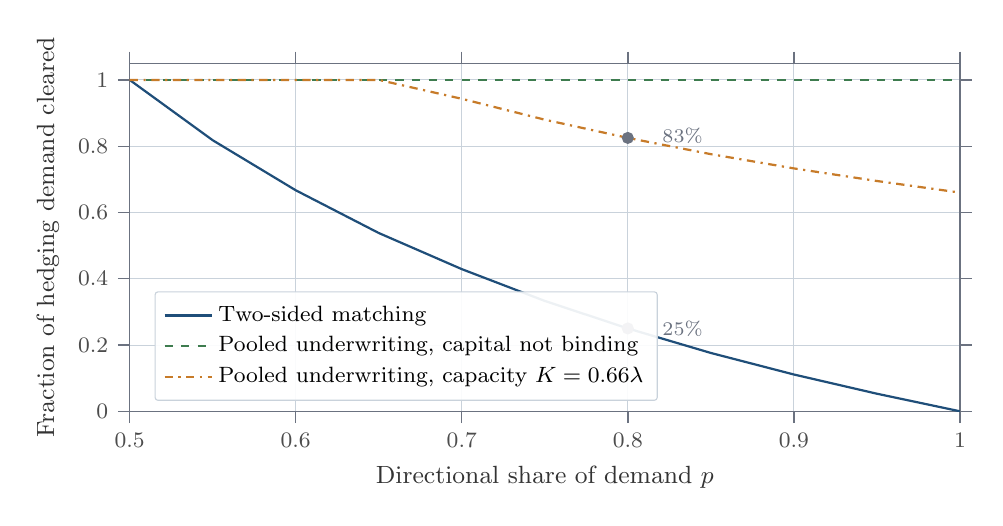
\begin{tikzpicture}
\begin{axis}[bzaxis,
  xlabel={Directional share of demand $p$},
  ylabel={Fraction of hedging demand cleared},
  xmin=0.5, xmax=1.0, ymin=0, ymax=1.05,
  xtick={0.5,0.6,0.7,0.8,0.9,1.0},
  ytick={0,0.2,0.4,0.6,0.8,1.0},
  legend pos=south west,
  height=6.0cm,
]
\addplot[bzblue, thick] coordinates {
 (0.50,1.000)(0.55,0.818)(0.60,0.667)(0.65,0.538)(0.70,0.429)
 (0.75,0.333)(0.80,0.250)(0.85,0.176)(0.90,0.111)(0.95,0.053)(1.00,0.000)};
\addlegendentry{Two-sided matching}

\addplot[bzgreen, thick, dashed] coordinates {(0.50,1.0)(1.00,1.0)};
\addlegendentry{Pooled underwriting, capital not binding}

\addplot[bzamber, thick, dash dot] coordinates {
 (0.50,1.000)(0.55,1.000)(0.60,1.000)(0.65,1.000)(0.70,0.943)
 (0.75,0.880)(0.80,0.825)(0.85,0.776)(0.90,0.733)(0.95,0.695)(1.00,0.660)};
\addlegendentry{Pooled underwriting, capacity $K = 0.66\lambda$}

\addplot[bzgray, only marks, mark=*, mark size=1.6pt] coordinates {(0.80,0.250)(0.80,0.825)};
\node[font=\scriptsize, anchor=west, bzgray] at (axis cs:0.815,0.25) {25\%};
\node[font=\scriptsize, anchor=west, bzgray] at (axis cs:0.815,0.83) {83\%};
\end{axis}
\end{tikzpicture}
\caption{Clearing under directional demand. At $p = 0.8$, which is a mild assumption for
regional weather hedging, a two-sided venue clears one hedger in four. A pooled venue clears
every hedger until reserved capital reaches the utilisation cap, and then degrades smoothly
rather than emptying. The capacity-bound curve is drawn for illustrative $K$; the derivation
of $K$ from protocol parameters is in Section~\ref{sec:capital}.}
\label{fig:clearing}
\end{figure}

\subsection{Why isolating markets is the wrong response}

The standard DeFi answer to risk concentration is to isolate pools, so that a failure in one
market cannot reach another. That answer is correct when markets are genuinely independent.
Weather markets are not. Rainfall in Tokyo and rainfall in Osaka in the same week can be the
same storm system. Isolation in that setting produces the appearance of diversification while
the underlying peril is shared, which is precisely the failure Miranda and Glauber identify
in crop insurance \cite{miranda1997}.

BreezeSwap therefore shares capital across markets and bounds the shared exposure explicitly,
rather than partitioning capital and hoping the partitions are meaningful.
Section~\ref{sec:correlation} describes the mechanism and reports what happens without it.

% ==================================================================
\section{Protocol design}
\label{sec:design}

\subsection{Three products, one balance sheet}

\begin{figure}[h]
\centering
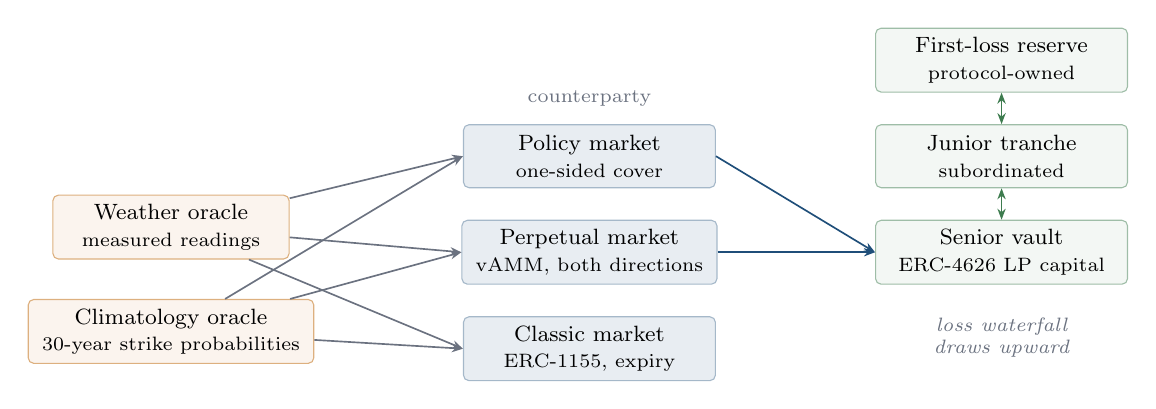
\begin{tikzpicture}[
  node distance=6mm,
  box/.style={draw=bzrule, fill=white, rounded corners=2pt, align=center,
              font=\footnotesize, minimum height=8mm, inner xsep=5pt},
  prod/.style={box, fill=bzlight, draw=bzblue!40, minimum width=32mm},
  capbox/.style={box, draw=bzgreen!50, fill=bzgreen!6, minimum width=32mm},
  ext/.style={box, draw=bzamber!60, fill=bzamber!8, minimum width=30mm},
  ar/.style={-{Stealth[length=4pt]}, bzgray, line width=0.6pt},
]

\node[ext] (oracle) {Weather oracle\\\scriptsize measured readings};
\node[ext, below=5mm of oracle] (clim) {Climatology oracle\\\scriptsize 30-year strike probabilities};

\node[prod, right=22mm of oracle, yshift=9mm] (policy) {Policy market\\\scriptsize one-sided cover};
\node[prod, below=4mm of policy] (perp) {Perpetual market\\\scriptsize vAMM, both directions};
\node[prod, below=4mm of perp] (classic) {Classic market\\\scriptsize ERC-1155, expiry};

\node[capbox,right=20mm of perp] (vault) {Senior vault\\\scriptsize ERC-4626 LP capital};
\node[capbox,above=4mm of vault] (junior) {Junior tranche\\\scriptsize subordinated};
\node[capbox,above=4mm of junior] (flr) {First-loss reserve\\\scriptsize protocol-owned};

\draw[ar] (oracle) -- (policy.west);
\draw[ar] (oracle) -- (perp.west);
\draw[ar] (oracle) -- (classic.west);
\draw[ar] (clim) -- (policy.west);
\draw[ar] (clim) -- (perp.west);
\draw[ar] (clim) -- (classic.west);

\draw[ar, bzblue] (policy.east) -- node[above, font=\scriptsize, bzgray, yshift=-1pt] {} (vault.west);
\draw[ar, bzblue] (perp.east) -- (vault.west);

\draw[{Stealth[length=4pt]}-{Stealth[length=4pt]}, bzgreen, line width=0.6pt] (vault) -- (junior);
\draw[{Stealth[length=4pt]}-{Stealth[length=4pt]}, bzgreen, line width=0.6pt] (junior) -- (flr);

\node[font=\scriptsize\itshape, bzgray, below=3mm of vault, align=center]
  {loss waterfall\\draws upward};

\node[font=\scriptsize, bzgray, above=1mm of policy, align=center]
  {counterparty};

\end{tikzpicture}
\caption{Product surface and capital stack. The classic market clears peer to peer and does
not consume vault capital; the policy and perpetual markets clear against the vault. All
three price against the same climatology feed, so a strike cannot be quoted in one product
at odds the protocol refuses in another.}
\end{figure}

\paragraph{Policy market.} A buyer pays a premium and receives a promise: if the aggregated
index over the covered period breaches a strike, the payout is transferred. This is the
Arbol-equivalent product, and it clears with one buyer because the vault underwrites it.

\paragraph{Perpetual market.} A trader takes long or short exposure to a weather index
against a virtual constant-product curve, with leverage capped at 3, a 10\% maintenance
margin, and funding that pulls the mark toward the oracle index. Positions can be closed at
any time, which is the property none of the insurance products offer.

\paragraph{Classic market.} An expiry-dated pool where both sides deposit collateral and
receive ERC-1155 position tokens that can be transferred or sold before settlement. Payoffs
may be binary, linear, or capped, and the calculator guarantees that the long and short
payouts sum exactly to the notional.

\subsection{The vAMM and why it needs a backstop}

The perpetual market prices against synthetic reserves $(x, y)$ satisfying $x \cdot y = k$,
with mark price $P = x/y$. No real assets sit in the curve. Opening a long increases $x$ and
decreases $y$; the trader's position size is the change in $y$.

This construction gives price discovery without liquidity providers posting into a curve,
which is exactly what a market with no natural two-sided flow needs. What it does not give
is a source of funds. In a matched book, one trader's profit is another's loss and the
market is self-funding. In a skewed book, the winning side's profit has no source, and
without a backstop the market pays it out of the collateral posted by traders who have not
yet closed, so the last trader to exit absorbs the shortfall.

\begin{keybox}{The core obligation}
A vAMM manufactures exposure, not capital. Every design that uses one either bounds the
skew it will accept, or backs the skew with real capital, or quietly makes its last exiting
trader the insurer of everyone before them. BreezeSwap does the first two and publishes the
bound.
\end{keybox}

Funding is the first line of defence and works on incentives: when the mark sits above the
oracle index, longs pay shorts, which makes the crowded side expensive to hold. Funding is
zero-sum only across matched open interest, so it cannot close a structural skew on its own.
The skew cap and the capital reserve do that.

\subsection{Three defects found by measurement}

Three implementation defects are worth recording because each was found by instrumenting the
system rather than by reading it, and each was invisible to tests that only checked whether
a call succeeded.

\begin{enumerate}[leftmargin=1.4em, itemsep=3pt]
\item \textbf{Oracle scale mismatch.} Mark price was 1e18-scaled and the oracle reading was
1e6-scaled. Nothing reconciled the two, so every funding calculation saw a deviation of
order $10^{16}$ basis points and clamped to the maximum rate in the same direction on every
call. Funding was not pulling the mark toward the index; it was a fixed maximum levy on
longs that no market condition could change. The market looked functional throughout.

\item \textbf{Settlement measuring a different quantity from pricing.} The climatology script
sums daily precipitation into a monthly total and counts how often that total breached the
strike, so a 40~mm threshold means 40~mm across the month. Settlement compared a single
reading at expiry against that threshold. One day of rainfall is almost always below a
monthly total, so drought cover triggered on nearly every policy while being charged the
monthly-total probability. The pricing was correct and the settlement was measuring
something else.

\item \textbf{Unbounded iteration on the payout path.} The function computing open-position
obligations looped over every position the market had ever created. That loop only grew, so
the sweep of realised trader losses to liquidity providers was guaranteed to exceed the block
gas limit eventually and stay there. It is a liveness failure on a timer, and no test that
opens a realistic number of positions would find it.
\end{enumerate}

Each now carries a regression test. The reason for listing them is that they are the class
of defect that separates a protocol that demonstrates well from one that holds capital
safely, and none of them is visible in an architecture diagram.

% ==================================================================
\section{Pricing weather}
\label{sec:pricing}

\subsection{Even odds is a transfer, not a simplification}

The premium for a binary weather claim is
\[
  \pi \;=\; L \cdot \hat{p} \cdot (1 + \lambda),
\]
where $L$ is the payout limit, $\hat{p}$ is the historical breach frequency for the specific
region, variable, direction, threshold, and calendar month, and $\lambda$ is the risk load.
The load is floored at 5\% and defaults to 30\%, with a further surcharge that scales with
how committed the pool is, capped at 50\% in total.

The floor exists because underwriting at historical fair value is a losing business. The
expected profit is zero by construction, and the realised outcome has variance, so a pool
charging exactly $L\hat{p}$ has a positive probability of ruin and a zero expected reward for
accepting it. Cao and Wei's empirical finding that the market price of weather risk is not
zero is the same statement from the other direction \cite{cao2004}.

Now compare against a contract collateralised at even odds, which is what a naive two-sided
pool implements. That contract charges $0.5L$ regardless of $\hat{p}$. The wedge is

\[
  \Delta(\hat p) \;=\; L\left(\hat{p} - 0.5\right),
\]

which is an expected transfer per unit of cover from the uninformed side to the informed one.

\begin{figure}[h]
\centering
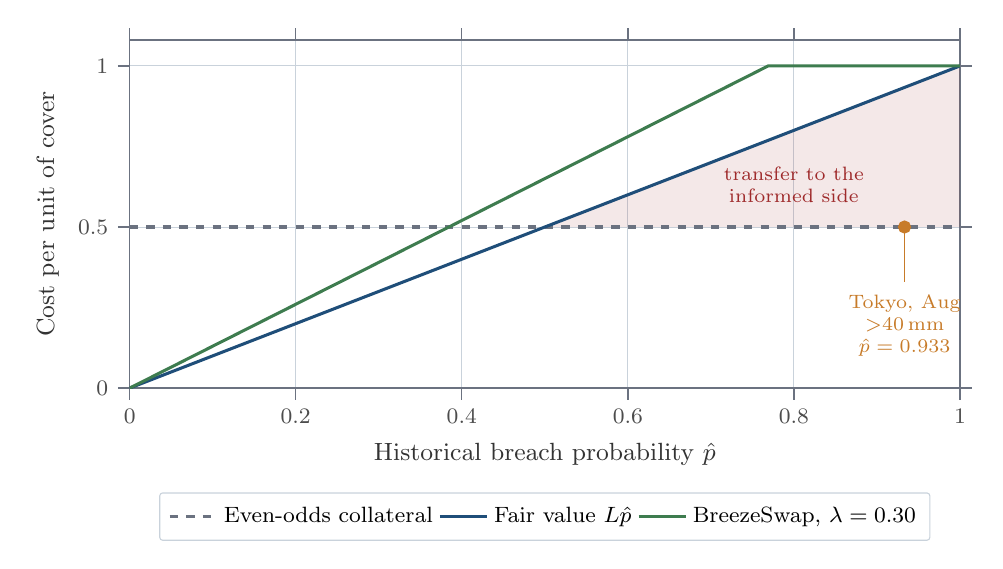
\begin{tikzpicture}
\begin{axis}[bzaxis,
  xlabel={Historical breach probability $\hat{p}$},
  ylabel={Cost per unit of cover},
  xmin=0, xmax=1, ymin=0, ymax=1.08,
  xtick={0,0.2,0.4,0.6,0.8,1.0},
  legend style={at={(0.5,-0.30)}, anchor=north, legend columns=3, draw=bzrule},
  height=6.0cm,
]
% Wedge between fair value and the even-odds line, drawn first so the curves sit on top.
\path[fill=bzred, fill opacity=0.11]
  (axis cs:0.5,0.5) -- (axis cs:1.0,1.0) -- (axis cs:1.0,0.5) -- cycle;

\addplot[bzgray, dashed] coordinates {(0,0.5)(1,0.5)};
\addlegendentry{Even-odds collateral}

\addplot[bzblue] coordinates {(0,0)(1,1)};
\addlegendentry{Fair value $L\hat{p}$}

\addplot[bzgreen] coordinates {(0,0)(0.769,1.0)(1,1.0)};
\addlegendentry{BreezeSwap, $\lambda = 0.30$}

\node[font=\scriptsize, bzred, anchor=center, align=center] at (axis cs:0.80,0.63)
  {transfer to the\\informed side};

\addplot[bzamber, only marks, mark=*, mark size=1.8pt, forget plot]
  coordinates {(0.9333,0.5)};
\draw[bzamber, line width=0.4pt] (axis cs:0.9333,0.485) -- (axis cs:0.9333,0.33);
\node[font=\scriptsize, bzamber, anchor=north, align=center] at (axis cs:0.9333,0.32)
  {Tokyo, Aug\\$>$40\,mm\\$\hat{p} = 0.933$};
\end{axis}
\end{tikzpicture}
\caption{Pricing a weather claim at even odds transfers value in proportion to how far the
true frequency sits from one half. On the Tokyo August 40~mm strike, where the threshold was
breached in 28 of 30 years, the transfer is 43.3 percentage points of the payout limit per
contract. The BreezeSwap premium tracks fair value with a floored load and is capped strictly
below the payout, so a buyer always retains something to win.}
\label{fig:premium}
\end{figure}

\subsection{The empirical record}

Strike probabilities are computed off-chain from the Open-Meteo archive
\cite{openmeteo}, which reanalyses observational data into a gridded historical record built
on ERA5 \cite{hersbach2020}. The seeded dataset used throughout this paper covers 1996 to
2025, thirty complete years, across five regions and nine thresholds for each calendar month
and each direction, producing 1{,}080 priced strikes. Each on-chain entry carries the sample
size behind it, and the contract refuses any entry derived from fewer than ten years.

Figure~\ref{fig:exceedance} shows why a single global threshold is meaningless. In August,
the probability that monthly rainfall exceeds 80~mm is 96.7\% in Singapore, 90.0\% in Seoul,
70.0\% in Tokyo, 16.7\% in London, and 0\% in Dubai. The same nominal contract is a near
certainty in one place and an impossibility in another.

\begin{figure}[h]
\centering
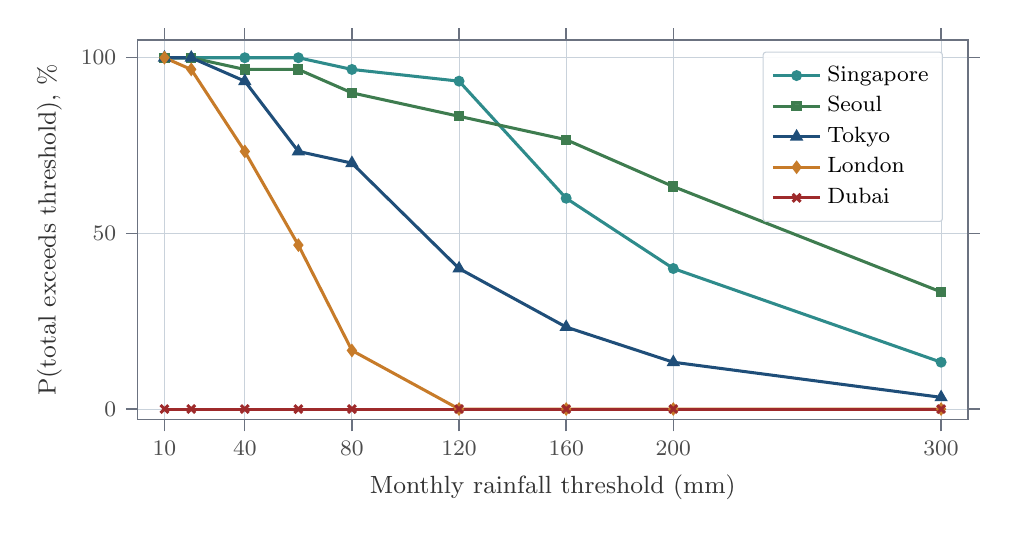
\begin{tikzpicture}
\begin{axis}[bzaxis,
  xlabel={Monthly rainfall threshold (mm)},
  ylabel={P(total exceeds threshold), \%},
  xmin=0, xmax=310, ymin=-3, ymax=105,
  xtick={10,40,80,120,160,200,300},
  legend pos=north east,
  height=6.4cm,
]
\addplot[bzteal, mark=*, mark size=1.4pt] coordinates {
 (10,100)(20,100)(40,100)(60,100)(80,96.67)(120,93.33)(160,60)(200,40)(300,13.33)};
\addlegendentry{Singapore}
\addplot[bzgreen, mark=square*, mark size=1.3pt] coordinates {
 (10,100)(20,100)(40,96.67)(60,96.67)(80,90)(120,83.33)(160,76.67)(200,63.33)(300,33.33)};
\addlegendentry{Seoul}
\addplot[bzblue, mark=triangle*, mark size=1.7pt] coordinates {
 (10,100)(20,100)(40,93.33)(60,73.33)(80,70)(120,40)(160,23.33)(200,13.33)(300,3.33)};
\addlegendentry{Tokyo}
\addplot[bzamber, mark=diamond*, mark size=1.6pt] coordinates {
 (10,100)(20,96.67)(40,73.33)(60,46.67)(80,16.67)(120,0)(160,0)(200,0)(300,0)};
\addlegendentry{London}
\addplot[bzred, mark=x, mark size=2pt] coordinates {
 (10,0)(20,0)(40,0)(60,0)(80,0)(120,0)(160,0)(200,0)(300,0)};
\addlegendentry{Dubai}
\end{axis}
\end{tikzpicture}
\caption{Empirical August exceedance curves, 1996 to 2025, from the seeded Open-Meteo
archive. Thirty observations per point. Dubai records no August month above 10~mm in the
sample, which is a correct answer and a reason the protocol will not list a market whose
strike has no informative history.}
\label{fig:exceedance}
\end{figure}

\subsection{Seasonality forces per-month pricing}

A single annual probability misprices every month. Figure~\ref{fig:seasonal} shows the
probability that Tokyo monthly rainfall exceeds 80~mm by calendar month: it runs from 23.3\%
in February to 96.7\% in June. A protocol pricing the annual average of 71.1\% would sell
February cover at roughly three times fair value and June cover at roughly three quarters of
it, and the second error is the expensive one because it is the one informed buyers will
take.

The strike key therefore includes the calendar month, and the month is derived on-chain from
the block timestamp rather than supplied as a parameter, so a market cannot be pointed at a
season whose climatology happens to flatter it.

\begin{figure}[h]
\centering
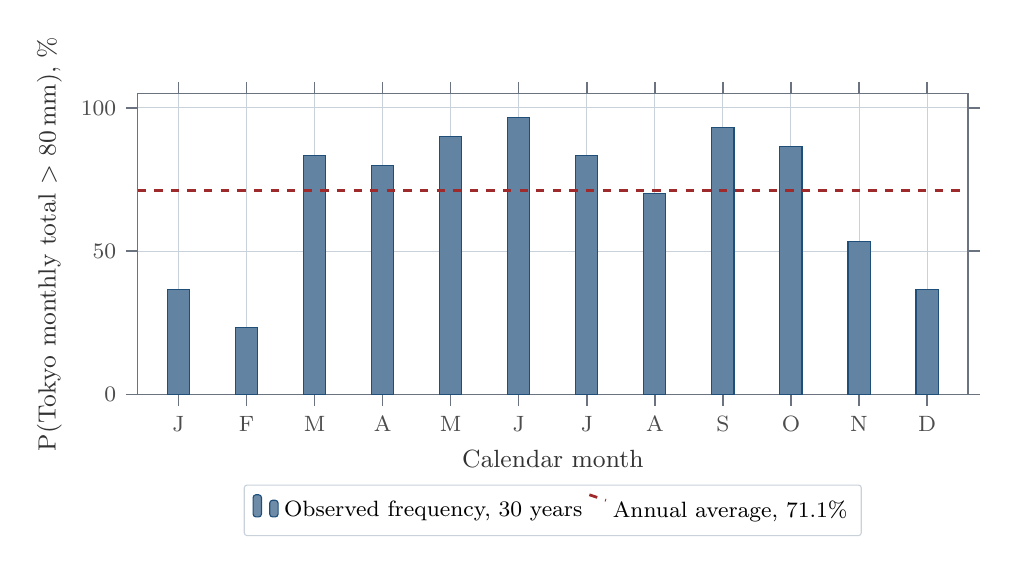
\begin{tikzpicture}
\begin{axis}[bzaxis,
  ybar,
  bar width=8pt,
  xlabel={Calendar month},
  ylabel={P(Tokyo monthly total $>$ 80\,mm), \%},
  xmin=0.4, xmax=12.6, ymin=0, ymax=105,
  xtick={1,2,3,4,5,6,7,8,9,10,11,12},
  xticklabels={J,F,M,A,M,J,J,A,S,O,N,D},
  height=5.4cm,
  legend style={at={(0.5,-0.30)}, anchor=north, legend columns=2, draw=bzrule},
  every axis plot/.append style={line width=0.4pt},
]
\addplot[draw=bzblue, fill=bzblue!70] coordinates {
 (1,36.67)(2,23.33)(3,83.33)(4,80)(5,90)(6,96.67)
 (7,83.33)(8,70)(9,93.33)(10,86.67)(11,53.33)(12,36.67)};
\addlegendentry{Observed frequency, 30 years}
\addplot[bzred, sharp plot, dashed, line width=1pt] coordinates {(0.4,71.1)(12.6,71.1)};
\addlegendentry{Annual average, 71.1\%}
\end{axis}
\end{tikzpicture}
\caption{Seasonality in a single strike. A protocol pricing off the annual average would
overcharge winter cover by a factor of three and undercharge June cover by a quarter.}
\label{fig:seasonal}
\end{figure}

\subsection{The distribution is skewed, so the mean is not the price}

Figure~\ref{fig:dist} plots the thirty August totals for Tokyo in ascending order. The mean
is 117.5~mm and the median is 104.7~mm; the standard deviation is 69.4~mm and the maximum,
315.5~mm, is 4.5 times the minimum. The distribution has a long right tail, which is the
normal shape for precipitation and the reason the protocol prices from empirical quantiles
rather than fitting a symmetric distribution and reading off a mean.

It is also the reason the risk load is not cosmetic. An underwriter selling exceedance cover
on this series is short the right tail, and the tail is where the capital goes.

\begin{figure}[h]
\centering
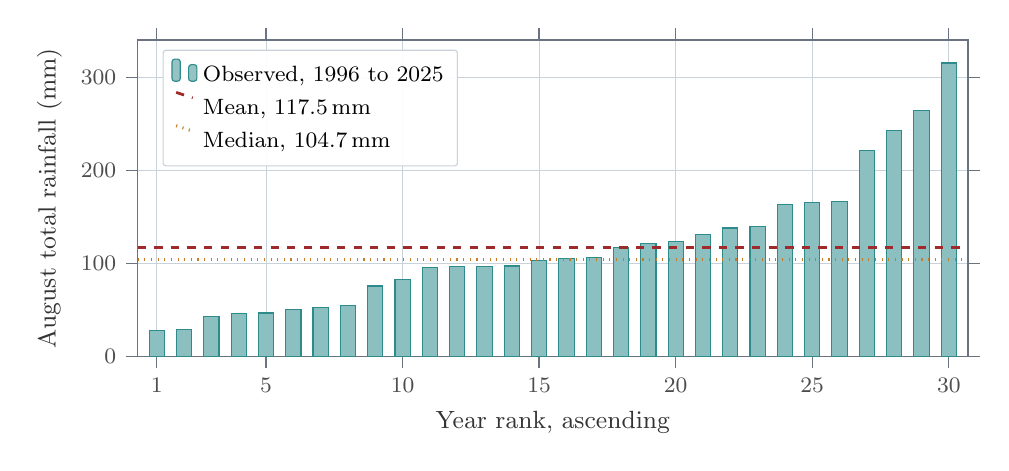
\begin{tikzpicture}
\begin{axis}[bzaxis,
  ybar,
  bar width=5.5pt,
  xlabel={Year rank, ascending},
  ylabel={August total rainfall (mm)},
  xmin=0.3, xmax=30.7, ymin=0, ymax=340,
  xtick={1,5,10,15,20,25,30},
  height=5.6cm,
  legend pos=north west,
  every axis plot/.append style={line width=0.4pt},
]
\addplot[draw=bzteal, fill=bzteal!55] coordinates {
 (1,28.3)(2,29.4)(3,42.8)(4,46.5)(5,46.8)(6,50.7)(7,52.3)(8,55)(9,75.9)(10,83.2)
 (11,96)(12,96.5)(13,97)(14,97.3)(15,103.7)(16,105.7)(17,106.4)(18,117.4)(19,121.5)(20,123.4)
 (21,130.8)(22,138.2)(23,139.7)(24,163.9)(25,165.6)(26,166.5)(27,221.1)(28,243.2)(29,264.4)(30,315.5)};
\addlegendentry{Observed, 1996 to 2025}
\addplot[bzred, sharp plot, dashed, line width=1pt] coordinates {(0.3,117.5)(30.7,117.5)};
\addlegendentry{Mean, 117.5\,mm}
\addplot[bzamber, sharp plot, dotted, line width=1.1pt] coordinates {(0.3,104.7)(30.7,104.7)};
\addlegendentry{Median, 104.7\,mm}
\end{axis}
\end{tikzpicture}
\caption{Tokyo August monthly rainfall totals, sorted. Mean above median, standard deviation
69.4~mm, and a maximum 4.5 times the minimum. Precipitation is right-skewed, so an
underwriter selling exceedance cover is short a tail rather than short a symmetric bet.}
\label{fig:dist}
\end{figure}

\subsection{Three gates, and what each refuses}

Pricing that lives only in a user interface is decoration. Each product therefore carries an
on-chain gate that can refuse a transaction outright, and Table~\ref{tab:gates} states what
each one turns away.

\begin{table}[htbp]
\centering
\small
\setlength{\tabcolsep}{6pt}
\renewcommand{\arraystretch}{1.3}
\begin{tabularx}{\linewidth}{@{}l>{\raggedright\arraybackslash}X>{\raggedright\arraybackslash}X@{}}
\toprule
\textbf{Product} & \textbf{Gate} & \textbf{What it refuses} \\
\midrule
Classic, binary & Fair-odds band on the long share of the pool & A deposit that pushes the
implied odds further from the historical frequency once already outside tolerance. A deposit
that moves the pool toward fair odds is always allowed, so a mispriced pool stays repairable. \\
Perpetual & Opening mark within a band of the climatological expected level for the month &
Market creation at a mark unrelated to the climate the index tracks, which would misprice
every subsequent trade. \\
Policy & Premium computed from the strike probability, load floored at 5\% &
Selling cover at or below expected loss, and any quote derived from fewer than ten years of
record. \\
\bottomrule
\end{tabularx}
\caption{Pricing gates by product. Linear and capped classic payoffs are deliberately left
unpriced: they require the loss distribution rather than a single quantile of it, and the
protocol flags them as unpriced on-chain rather than attaching an authoritative-looking
wrong number.}
\label{tab:gates}
\end{table}

\subsection{Adverse selection and the sale window}

Historical frequency is an unconditional probability. A buyer who can see a forecast of the
period being covered holds a conditional probability instead, and will buy only when the
conditional exceeds the price. That is not bad luck for the pool; it is systematic bleed, and
it is the mechanism Rothschild and Stiglitz describe \cite{rothschild1976}.

Numerical weather prediction carries real skill to roughly two weeks, with marginal skill
extending to about six \cite{bauer2015}. The protocol therefore refuses to sell cover whose
covered period begins sooner than a configured lead time, defaulting to 45 days and floored
at 21 days so the parameter cannot be tuned back inside the forecast horizon. This is the
same instrument as a crop insurance sales closing date, expressed as a contract condition
rather than an underwriting policy.

\subsection{Settlement must measure what pricing measured}

If the premium was derived from the frequency with which a monthly total breached a
threshold, then settlement must compare a monthly total against that threshold. Each policy
therefore records an aggregation at purchase, summing readings for rainfall totals and
averaging them for temperature means, and settlement collapses the whole covered period using
the recorded statistic rather than reading a single value at expiry.

Two further conditions follow. Readings are sampled on an exact grid and a reading whose
timestamp does not match is treated as absent rather than substituted, because an oracle that
falls back to the most recent value would silently contribute the previous day twice into a
sum. And a settlement requires at least 93\% of expected samples to be present, matching the
tolerance the climatology script applies when it discards incomplete months. The tolerance is
tight in this direction specifically: a missing sample under-counts a total, which biases
drought cover toward paying out, so the error favours the buyer and it is the capital
providers who need the bound.

% ==================================================================
\section{Capital economics}
\label{sec:capital}

This is the section that determines whether the protocol works with less liquidity than its
competitors or merely claims to.

\subsection{What the protocol locks, and why gross}

For policy cover the vault reserves the gross payout limit, not the limit net of premium.
Reserving net looks correct, since the premium is paid in and the two together appear to
cover the promise. They do not, for a timing reason. Premium becomes recognised liquidity
provider value on a vesting schedule with no relation to the policy's term, while the
obligation runs to expiry. A claim then arrives short by exactly the premium, and the effect
grows with the strike probability: on a strike with a 70\% breach frequency the premium is
most of the payout, so almost nothing would be reserved and the cover would be largely
notional. Cover is collateralised to its full limit, as a catastrophe bond is
\cite{froot2001}.

For perpetual markets the reserve requirement is a fraction of worst-case directional
notional rather than the whole of it, because a perpetual position's loss is bounded by price
movement rather than by a binary payout. Two choices in that definition are load-bearing.

\paragraph{Worst case, not current skew.} The requirement is sized on
$\max(N_{\text{long}}, N_{\text{short}})$, not on $|N_{\text{long}} - N_{\text{short}}|$. A
balanced book of 100k against 100k has zero skew and would reserve nothing, but the moment
one side closes the imbalance is 100k, and by then the capital providers whose funds would
have backed it have already been free to withdraw. Sizing on the larger side prices the
exposure the book can reach without a single new position opening.

\paragraph{Preventive, not reactive.} Capacity is derived from backing that already exists
and an opening trade is refused before any token moves, so an under-reserved state is
unrepresentable rather than merely detectable. Exits are never gated by capacity, which
matters because a book pushed over its cap by a tightened parameter or a capital provider
withdrawal must stay repairable.

\subsection{Deriving the capital multiplier}

Let $S$ be senior vault assets, $J$ junior tranche assets, $u$ the aggregate utilisation cap,
$c$ the single-market concentration cap, $\sigma$ the coverage ratio applied to worst-case
notional, and $\beta$ the maximum share of counted backing that junior capital may supply.
The shipped parameters are
\[
  u = 0.80,\quad c = 0.50,\quad \sigma = 0.50,\quad \beta = 0.3333 .
\]

Counted backing is senior assets plus credited junior assets, where credit is capped so that
junior can never exceed $\beta$ of the total. Solving $c_J \le \beta(S + c_J)$ gives
\[
  B \;=\; S + \min\!\left(J,\; \frac{\beta}{1-\beta}\,S\right)
  \;\le\; \frac{S}{1-\beta} \;=\; 1.50\,S .
\]

The reserve a market must hold against worst-case notional $N$ is $\sigma N$. Summed across
markets the utilisation cap gives
\[
  \sigma \sum_i N_i \;\le\; u B
  \quad\Longrightarrow\quad
  \sum_i N_i \;\le\; \frac{u}{\sigma}\,B \;=\; 1.6\,B \;\le\; 2.40\,S ,
\]
and for any single market the concentration cap binds first:
\[
  N_{\text{single}} \;\le\; \frac{c}{\sigma}\,B \;=\; 1.0\,B \;\le\; 1.50\,S .
\]

For policy cover the binding constraints are an aggregate outstanding-payout cap of 60\% of
senior assets and a per-peril cap of 20\%, so a pool of size $S$ supports $0.6S$ of
outstanding limit spread across at least three distinct region-months.

\begin{keybox}{The multiplier, stated plainly}
One unit of senior capital supports up to 2.40 units of worst-case directional notional
across the perpetual markets, or 1.50 units if a single market is the whole book, and 0.60
units of fully collateralised policy limit outstanding at any moment. The perpetual figures
require the junior tranche to be subscribed to its counted share; without it they are 1.60
and 1.00 respectively.
\end{keybox}

\begin{figure}[h]
\centering
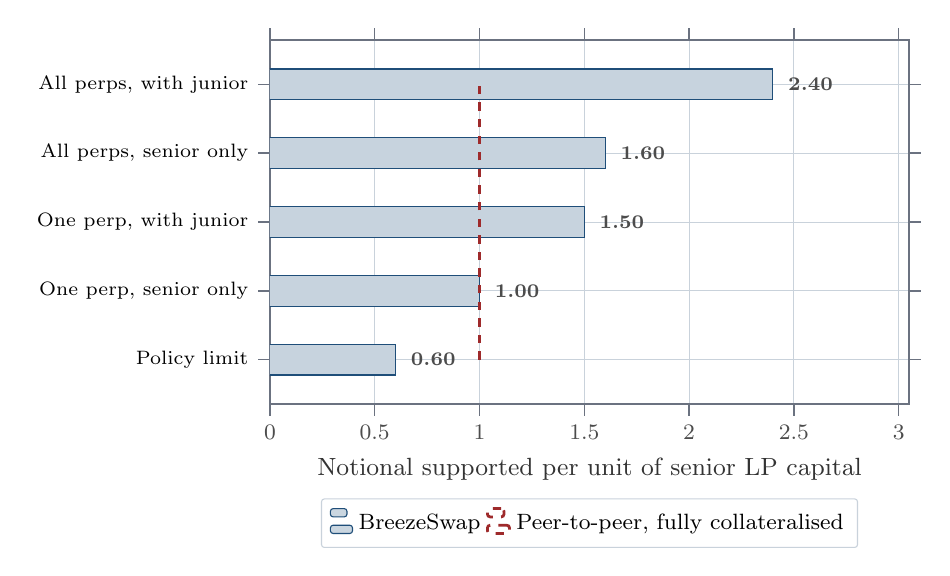
\begin{tikzpicture}
\begin{axis}[bzaxis,
  xbar,
  bar width=11pt,
  width=0.80\linewidth,
  xlabel={Notional supported per unit of senior LP capital},
  xmin=0, xmax=3.05,
  enlarge y limits=0.16,
  ytick=data,
  symbolic y coords={
    {Policy limit},
    {One perp, senior only},
    {One perp, with junior},
    {All perps, senior only},
    {All perps, with junior}},
  yticklabel style={font=\scriptsize, align=right},
  nodes near coords,
  nodes near coords style={font=\scriptsize\bfseries, color=black!70, xshift=2pt},
  nodes near coords align={anchor=west},
  point meta=explicit symbolic,
  height=6.2cm,
  every axis plot/.append style={line width=0.4pt},
  legend style={at={(0.5,-0.26)}, anchor=north, legend columns=2, draw=bzrule},
]
\addplot[draw=bzblue, fill=bzblue!25] coordinates {
  (0.60,{Policy limit})             [0.60]
  (1.00,{One perp, senior only})    [1.00]
  (1.50,{One perp, with junior})    [1.50]
  (1.60,{All perps, senior only})   [1.60]
  (2.40,{All perps, with junior})   [2.40]};
\addlegendentry{BreezeSwap}
\addplot[bzred, sharp plot, dashed, line width=1pt, forget plot, nodes near coords={}]
  coordinates {
  (1.0,{Policy limit})
  (1.0,{All perps, with junior})};
\addlegendimage{bzred, dashed, line width=1pt}
\addlegendentry{Peer-to-peer, fully collateralised}
\end{axis}
\end{tikzpicture}
\caption{Capital multiplier by constraint, derived from the shipped parameters. The dashed
line is a fully collateralised peer-to-peer contract, which supports exactly one unit of
notional per unit of capital and additionally requires a matched counterparty to exist.
Note the honest reading: policy cover is \emph{less} capital-efficient than a bilateral
contract, at 0.60. Its advantage is that it clears at all.}
\label{fig:multiplier}
\end{figure}

\subsection{What this means for capital providers}

The gross expected return on senior capital from policy underwriting, at full use of the
aggregate cap, is
\[
  r \;=\; \underbrace{0.60}_{\text{aggregate cap}} \times
          \underbrace{\frac{365}{T}}_{\text{turnover}} \times
          \hat{p} \times \lambda ,
\]
where $T$ is the cover term in days. At the protocol's binding term limit of 62 days under
daily sampling and the default 30\% load, this is $r \approx 1.06\,\hat{p}$ per year.

\begin{table}[h]
\centering
\small
\setlength{\tabcolsep}{9pt}
\renewcommand{\arraystretch}{1.25}
\begin{tabular}{@{}lccc@{}}
\toprule
Strike breach probability $\hat{p}$ & 0.10 & 0.20 & 0.30 \\
\midrule
Expected premium per unit of limit & 0.130 & 0.260 & 0.390 \\
Expected loss per unit of limit & 0.100 & 0.200 & 0.300 \\
Expected margin per unit of limit & 0.030 & 0.060 & 0.090 \\
Gross annual return on senior capital & 10.6\% & 21.2\% & 31.8\% \\
\bottomrule
\end{tabular}
\caption{Gross expected return on senior capital from policy underwriting, at full use of the
aggregate exposure cap, 62-day terms, and the default 30\% risk load. These are expectations
before variance, before protocol fees, and before any allowance for the periods in which the
book is not at the cap. A pool writing high-probability strikes earns more in expectation and
pays claims far more often, so the variance of the realised path rises with $\hat{p}$ as well.}
\end{table}

The number that makes this interesting is not its level but its correlation. Weather risk is
close to uncorrelated with crypto asset returns, so a vault whose drawdowns are driven by
rainfall does not draw down at the same moment as the rest of a DeFi portfolio. That is an
unusual property in on-chain yield and it is the reason capital has a reason to arrive at all.

% ==================================================================
\section{The loss waterfall}
\label{sec:waterfall}

\subsection{Structure}

A loss that a market cannot fund is drawn in a fixed order, and each tier's contribution is
emitted so the ordering is verifiable from outside the contract.

\begin{figure}[h]
\centering
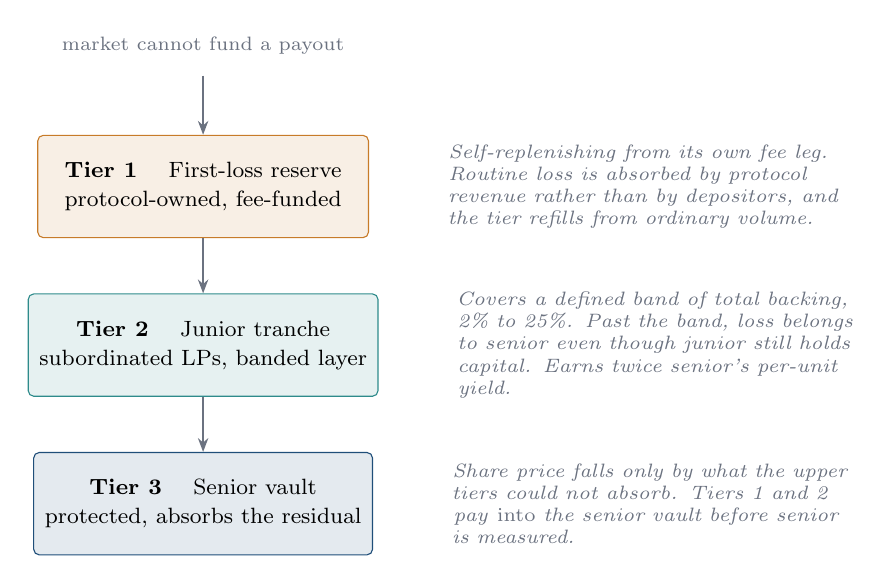
\begin{tikzpicture}[
  tier/.style={draw, rounded corners=2pt, align=center, font=\footnotesize,
               minimum width=42mm, minimum height=13mm, inner sep=4pt},
  lbl/.style={font=\scriptsize\itshape, color=bzgray, align=left},
  ar/.style={-{Stealth[length=5pt]}, bzgray, line width=0.7pt},
]
\node[tier, draw=bzamber, fill=bzamber!12] (t1)
  {\textbf{Tier 1} \quad First-loss reserve\\[1pt]protocol-owned, fee-funded};
\node[tier, draw=bzteal, fill=bzteal!12, below=7mm of t1] (t2)
  {\textbf{Tier 2} \quad Junior tranche\\[1pt]subordinated LPs, banded layer};
\node[tier, draw=bzblue, fill=bzblue!12, below=7mm of t2] (t3)
  {\textbf{Tier 3} \quad Senior vault\\[1pt]protected, absorbs the residual};

\draw[ar] (t1) -- (t2);
\draw[ar] (t2) -- (t3);

\node[lbl, right=9mm of t1, text width=50mm]
  {Self-replenishing from its own fee leg. Routine loss is absorbed by protocol revenue
   rather than by depositors, and the tier refills from ordinary volume.};
\node[lbl, right=9mm of t2, text width=50mm]
  {Covers a defined band of total backing, 2\% to 25\%. Past the band, loss belongs to
   senior even though junior still holds capital. Earns twice senior's per-unit yield.};
\node[lbl, right=9mm of t3, text width=50mm]
  {Share price falls only by what the upper tiers could not absorb. Tiers 1 and 2 pay
   \emph{into} the senior vault before senior is measured.};

\node[font=\scriptsize, bzgray, above=9mm of t1] {market cannot fund a payout};
\draw[ar] ($(t1.north)+(0,7.5mm)$) -- (t1.north);
\end{tikzpicture}
\caption{The three-tier loss waterfall. Both upper tiers are optional; with neither
configured the structure collapses to single-pool behaviour and the depositor interface is
unchanged.}
\end{figure}

Two design points deserve emphasis. Tier 2 is a layer, not a bucket: attachment and
exhaustion points are expressed as fractions of total backing, and the width becomes a
per-period aggregate limit, so junior's exposure is bounded in time and therefore priceable.
And tier 1 has its own dedicated balance rather than sharing one with the liquidation
backstop, because sharing let the vault drain the reserve that liquidation depends on.

\subsection{Tranching redistributes loss, it does not reduce it}

The claim that a subordinated tranche protects senior capital is comparative, so testing it
requires a comparative experiment: the same trader flow, from the same seed, run through
capital structures holding the same total risk capital. A structure that is safer because it
is simply larger has demonstrated nothing about tranching.

The simulation runs four arms over 40 traders, 6 capital providers, and 250 actions per seed
across 5 seeds, with 400{,}000 units of total capital:

\begin{itemize}[leftmargin=1.4em, itemsep=2pt]
\item \textbf{Arm A}: single tranche, 400k senior. The pre-waterfall baseline.
\item \textbf{Arm C}: 300k senior plus 100k junior, carved out of the same total.
\item \textbf{Arm D}: 400k senior plus 100k \emph{additional} junior.
\end{itemize}

\begin{figure}[h]
\centering
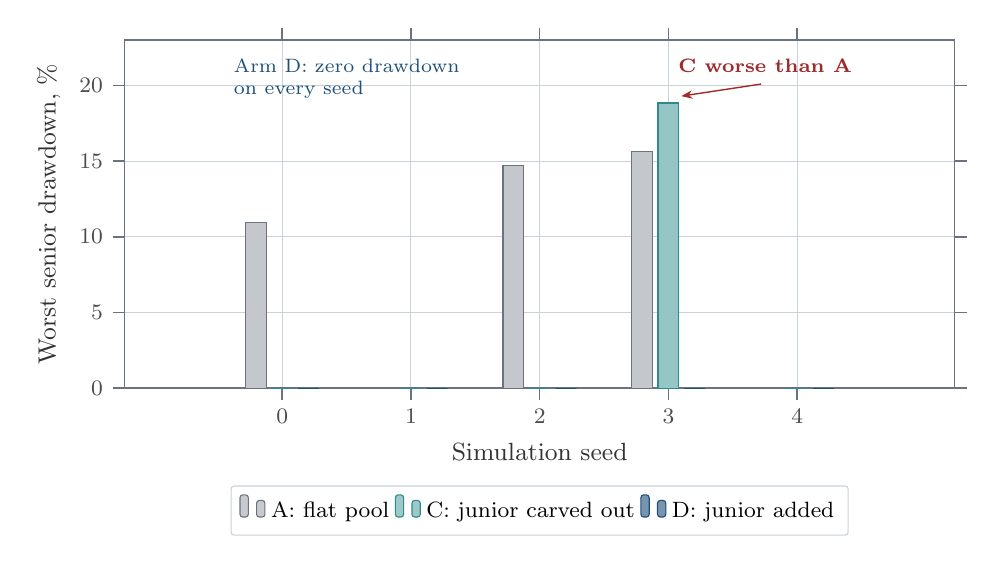
\begin{tikzpicture}
\begin{axis}[bzaxis,
  ybar,
  bar width=7.5pt,
  xlabel={Simulation seed},
  ylabel={Worst senior drawdown, \%},
  xmin=-0.6, xmax=4.6, ymin=0, ymax=23,
  xtick={0,1,2,3,4},
  ytick={0,5,10,15,20},
  height=6.0cm,
  legend style={at={(0.5,-0.28)}, anchor=north, legend columns=3, draw=bzrule},
  every axis plot/.append style={line width=0.4pt},
  enlarge x limits=0.12,
]
\addplot[draw=bzgray, fill=bzgray!40] coordinates {
 (0,10.93)(1,0)(2,14.71)(3,15.64)(4,0)};
\addlegendentry{A: flat pool}
\addplot[draw=bzteal, fill=bzteal!50] coordinates {
 (0,0)(1,0)(2,0)(3,18.85)(4,0)};
\addlegendentry{C: junior carved out}
\addplot[draw=bzblue, fill=bzblue!65] coordinates {
 (0,0)(1,0)(2,0)(3,0)(4,0)};
\addlegendentry{D: junior added}

\node[font=\scriptsize, bzblue, anchor=north west, align=left] at (axis cs:-0.45,22.4)
  {Arm D: zero drawdown\\on every seed};
\node[font=\scriptsize\bfseries, bzred, anchor=north east, align=right] at (axis cs:4.5,22.4)
  {C worse than A};
\draw[bzred, -{Stealth[length=4pt]}, line width=0.5pt]
  (axis cs:3.72,20.1) -- (axis cs:3.10,19.3);
\end{axis}
\end{tikzpicture}
\caption{Worst senior drawdown by arm and seed, measured as the largest fall in senior share
price from its starting value of 1.0. Arm C beats the flat pool on four seeds and loses on
seed 3, where a senior tranche 25\% thinner moves further per unit of residual loss once
junior is exhausted. Arm D, where junior capital is genuinely additional, never draws down at
all. Mean drawdown: A 8.26\%, C 3.77\%, D 0.00\%.}
\label{fig:waterfall}
\end{figure}

Seed 3 is the whole result. Arm C's worst senior share price of 0.8115 is worse than the flat
pool's 0.8436, because once the junior layer is exhausted the residual falls on a senior
tranche that is 25\% smaller. Tranching moved the loss; it did not remove it.

\begin{keybox}{Why junior capital must be additive, and how that is enforced}
A vault cannot control where a depositor's money came from, so ``additive'' cannot be
enforced at the point of deposit. What it can control is whether junior capital \emph{buys
capacity}. Counting junior toward backing only up to $\beta = 1/3$ of the total means a
protocol that funds itself by moving senior depositors into the junior tranche gets no extra
capacity for it, while one that attracts genuinely new subordinated capital does. Excess
junior capital is not rejected and not trapped: it still absorbs loss, and it stays
withdrawable, because capital that backs no capacity cannot be holding any up.
\end{keybox}

A separate arm measured whether tier 1 alone helps. Across five seeds the dedicated
first-loss reserve improved the mean worst senior share price from 0.9174 to 0.9300 and was
drawn on three of five seeds, with no seed made worse. When the same tier shared a balance
with the liquidation backstop rather than holding its own, it measured worse for senior than
having no tier 1 at all on two of five seeds.

% ==================================================================
\section{Calibrating the reserve}
\label{sec:calibration}

\subsection{The trade-off}

The coverage ratio $\sigma$ sets how much of worst-case directional notional must be backed
by capital. Raising it makes shortfalls less likely and rejects more trades. Lowering it does
the reverse, up to a point: a pool that drains rejects everything, so under-reserving is
capable of being worse on both axes at once.

The sweep runs three seeds of 900 actions each under the most aggressive funding parameters
the protocol permits. That preset is chosen deliberately. Under production funding parameters
every ratio including 30\% survives, so that regime cannot discriminate; it shows the protocol
is comfortable, not that 30\% is safe. Insurance capital is sized on the tail.

\begin{figure}[h]
\centering
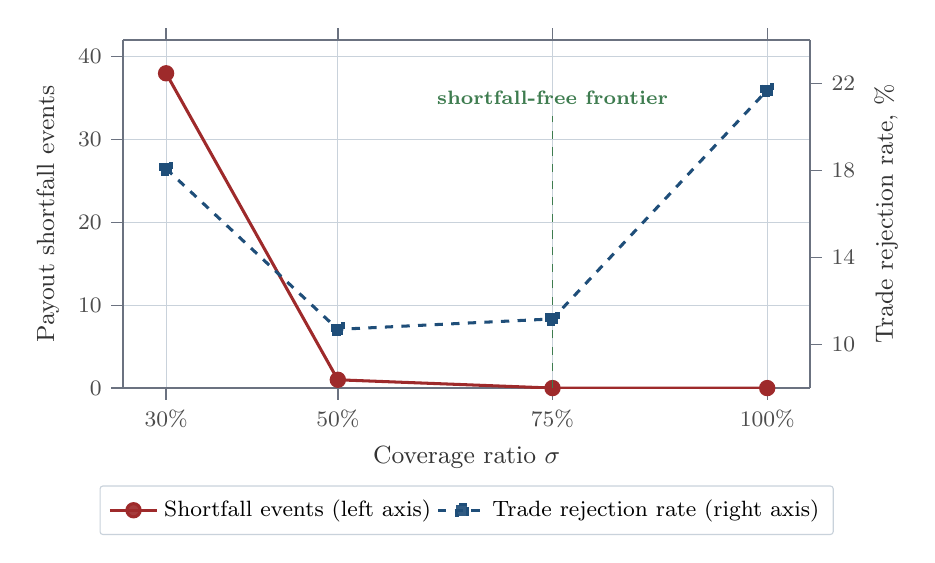
\begin{tikzpicture}
\begin{axis}[bzaxis,
  width=0.85\linewidth,
  xlabel={Coverage ratio $\sigma$},
  ylabel={Payout shortfall events},
  axis y line*=left,
  xmin=25, xmax=105, ymin=0, ymax=42,
  xtick={30,50,75,100},
  xticklabels={30\%,50\%,75\%,100\%},
  height=6.0cm,
  legend style={at={(0.5,-0.28)}, anchor=north, legend columns=2, draw=bzrule},
]
\addplot[bzred, mark=*, mark size=2.4pt] coordinates {(30,38)(50,1)(75,0)(100,0)};
\addlegendentry{Shortfall events (left axis)}
\addlegendimage{bzblue, mark=square*, mark size=2pt, dashed}
\addlegendentry{Trade rejection rate (right axis)}
\end{axis}
\begin{axis}[bzaxis,
  width=0.85\linewidth,
  axis y line*=right,
  axis x line=none,
  ylabel={Trade rejection rate, \%},
  xmin=25, xmax=105, ymin=8, ymax=24,
  ytick={10,14,18,22},
  height=6.0cm,
  grid=none,
]
\addplot[bzblue, mark=square*, mark size=2pt, dashed] coordinates {
 (30,18.09)(50,10.70)(75,11.18)(100,21.70)};
\draw[bzgreen, line width=0.7pt, dashed] (axis cs:75,8) -- (axis cs:75,20.5);
\node[font=\scriptsize\bfseries, bzgreen, anchor=south] at (axis cs:75,20.6)
  {shortfall-free frontier};
\end{axis}
\end{tikzpicture}
\caption{Reserve coverage sweep, 3 seeds by 900 actions under the aggressive funding preset.
At 30\% the pool both fails to pay traders and rejects more trades than at 50\%, because a
drained pool refuses everything. The shipped setting of 50\% produced one shortfall event
with a worst severity of 30.9\% of the amount owed. At 75\% shortfalls disappear at a cost of
0.48 percentage points of additional rejection.}
\label{fig:calib}
\end{figure}

\begin{table}[h]
\centering
\small
\setlength{\tabcolsep}{8pt}
\renewcommand{\arraystretch}{1.25}
\begin{tabular}{@{}lcccc@{}}
\toprule
Coverage ratio & 30\% & \textbf{50\% (shipped)} & 75\% & 100\% \\
\midrule
Shortfall events & 38 & \textbf{1} & 0 & 0 \\
Worst shortfall, \% of amount owed & 100.0 & \textbf{30.9} & 0 & 0 \\
Mean trade rejection rate & 18.09\% & \textbf{10.70\%} & 11.18\% & 21.70\% \\
Seeds ending near-drained & 2 of 3 & \textbf{0} & 0 & 0 \\
\bottomrule
\end{tabular}
\caption{Reserve calibration sweep, measured. Under-reserving is dominated: 30\% is worse on
both the solvency axis and the liquidity axis. The interesting comparison is 50\% against
75\%, where 0.48 percentage points of extra rejection buys the elimination of the remaining
shortfall.}
\label{tab:calib}
\end{table}

\subsection{The result argues against the shipped parameter}

We report this rather than round it away. The protocol currently ships $\sigma = 0.50$, and
under the aggressive funding preset that setting produced one shortfall event across 2{,}700
simulated actions, with a worst severity of 30.9\% of the amount a trader was owed. Setting
$\sigma = 0.75$ eliminated it and cost 0.48 percentage points of additional trade rejection.

The reserve calibration also has a known hole: 40\% was not tested, so the failure boundary
is only located somewhere between 30\% and 50\%. Section~\ref{sec:limits} carries both points
forward as open items rather than resolving them here.

\subsection{Scarcity is priced, not only rationed}

A hard capacity cap is a cliff. Below it every trade costs the same; at it, nothing gets
through. That is the wrong shape for a scarce resource, because it neither discourages the
marginal trade that fills the last of the book nor pays capital providers more for the tail
exposure they take as the book fills.

The protocol therefore charges a surcharge that scales linearly with capacity utilisation,
from zero on an empty book to 0.40\% of collateral on a full one, applied only to flow that
raises worst-case exposure. A trade that grows the smaller side consumes no scarce capacity
and pays nothing extra. The proceeds are retained in the market, which puts its balance above
open-position obligations, so the existing surplus sweep remits them to capital providers.

The surcharge does not replace the cap. The cap is a solvency bound derived from capital that
exists; the surcharge makes the approach to it expensive so the cliff binds less often.
Removing the cap and relying on price would mean accepting exposure the capital cannot
support at any fee.

% ==================================================================
\section{Correlated exposure}
\label{sec:correlation}

Two rainfall markets on regions that see the same storm system are not two risks. Each
market's own capacity bounds it against the shared pool, but nothing bounded the correlated
set, so both could fill their allowance against a single weather event.

Measured without a group cap, two correlated rainfall markets committed 599{,}400 against a
1{,}000{,}000 pool, a 50\% overshoot of what any single peril's cap permits. The registry
buckets markets by declared peril and takes the tighter of a market's own capacity and what
its peril group leaves it.

Exposure is pulled from registered markets rather than mirrored in registry state. Push
accounting would require every open, close, and liquidation to update a copy of state that
already exists, and any missed path leaves the copy wrong in a way nothing detects. Pulling
cannot desynchronise because there is nothing to synchronise. The loop is bounded by a
governance-set maximum, which is what keeps a correctness mechanism from becoming a gas trap.

Three properties hold throughout. A cap refuses a trade only when it actually raises
worst-case exposure, so a balancing trade is accepted even while the book is over its cap.
Exits are never gated. And a registry that reverts degrades to the market's own capacity
rather than blocking trading, because a correctness improvement must not become a liveness
failure.

\begin{table}[h]
\centering
\small
\setlength{\tabcolsep}{7pt}
\renewcommand{\arraystretch}{1.25}
\begin{tabular}{@{}lcl@{}}
\toprule
\textbf{Limit} & \textbf{Setting} & \textbf{Binds on} \\
\midrule
Aggregate vault utilisation & 80\% of backing & All reservations, both product lines \\
Ceiling on that cap & 90\% & Immutable; no admin action raises it \\
Single-market concentration & 50\% of backing & One market's reservation \\
Policy aggregate outstanding & 60\% of senior assets & Total payout limit written \\
Policy per-peril outstanding & 20\% of senior assets & One region-month bucket \\
Underwriting halt & 70\% utilisation & New policy sales only \\
Perp open-interest skew & 25\% of initial reserve & Unmatched open interest \\
Junior share of counted backing & 33.33\% & Capacity credit, not loss absorption \\
\bottomrule
\end{tabular}
\caption{Exposure limits. Each is a separate bound and the tightest one governs. The
underwriting halt sits deliberately below the vault's own reservation ceiling so the pool
keeps a solvency buffer rather than writing cover down to the last unit, which is the role a
minimum capital requirement plays in a mutual \cite{nexus_mutual}.}
\end{table}

% ==================================================================
\section{Protecting capital providers from each other}

Three mechanisms exist because a pooled vault creates opportunities to extract value from
other depositors that a bilateral contract does not.

\paragraph{Premium vests, it does not land.} Premium is earned across the life of the risk it
pays for. Crediting it at the moment of sale would let a depositor arrive one block before a
sale, capture the whole premium through the jump in share price, and leave the next block
having carried none of the exposure. Recognition is linear over a configurable period,
defaulting to seven days and floored at one, and the vesting deadline is stored explicitly so
that repeated trivial deposits cannot restart the clock on premium already part-way through
vesting.

\paragraph{Exit is delayed, never blocked.} Losses hit share price the moment a claim settles,
while profit is recognised gradually, and the oracle reading that triggers a claim is public
before anybody calls settlement. Without a delay a depositor can read the trigger and exit
ahead of settlement, leaving the loss with whoever stayed, which would make underwriting
optional for the well-informed and compulsory for everyone else. A withdrawal request starts a
cooldown, defaulting to three days and capped at fourteen, and the request snapshots the share
balance held at request time so a pre-warmed empty address is worth nothing. Any outbound
share transfer cancels the request. The cooldown in force is snapshotted with the request, so
a later increase cannot retroactively freeze somebody who has already begun waiting.

\paragraph{Pausing never traps funds.} Deposits are pausable and withdrawals are not.
Opening a position is pausable; closing and liquidating are not. An emergency control that
strands user collateral is not a safety mechanism.

% ==================================================================
\section{Empirical validation}
\label{sec:validation}

Every figure below was produced by running the repository's suites at the commit this paper
describes, not quoted from documentation.

\begin{table}[h]
\centering
\small
\setlength{\tabcolsep}{9pt}
\renewcommand{\arraystretch}{1.25}
\begin{tabular}{@{}lr@{}}
\toprule
\textbf{Measure} & \textbf{Result} \\
\midrule
Test suites & 54 \\
Tests passing & 568 of 568 \\
Tests failing & 0 \\
Wall-clock runtime & 114.9 s \\
Solidity contracts & 29 \\
Invariant runs & 256 runs at depth 64 \\
Fuzz iterations & 10{,}000 per property \\
Priced strikes in the seeded climatology & 1{,}080 \\
Years of observational record per strike & 30 \\
\bottomrule
\end{tabular}
\caption{Suite results, measured. The full command is \code{forge test --summary} from the
\code{contracts} directory.}
\end{table}

The suites that carry the claims in this paper are named rather than aggregated:

\begin{itemize}[leftmargin=1.4em, itemsep=2pt]
\item \code{ReserveMonteCarloTest} produces Table~\ref{tab:calib} and Figure~\ref{fig:calib}.
\item \code{WaterfallMonteCarloTest} produces Figure~\ref{fig:waterfall}.
\item \code{PerilAggregationTest}, 19 tests, covers the correlated exposure caps including
the requirement that a balancing trade is accepted over the cap and that a broken registry
does not block trading.
\item \code{PerpCapacityCapTest}, 14 tests, covers preventive capacity.
\item \code{FirstLossIsolationTest}, 12 tests, covers the separation of tier 1 from the
liquidation backstop.
\item \code{PerpFundingScaleTest}, 29 tests, is the regression suite for the oracle scale
defect.
\item \code{NightmareScenariosTest} covers named worst cases, including the bank-run path
that exposed the interaction between senior withdrawals and credited junior backing.
\end{itemize}

The invariants under continuous test are that market collateral plus insurance reserves cover
aggregate open position equity; that the constant product $k$ is preserved across every open
and close; that cumulative funding payments balance exactly between longs and shorts; that
long and short payouts sum to notional in every payoff mode; and that no path creates value
or permanently strands funds.

% ==================================================================
\section{Limitations and status}
\label{sec:limits}

This section is deliberately specific. A whitepaper that does not state what is missing is
not describing a system, it is advertising one.

\paragraph{The only functioning weather oracle is a mock.} The FTSO and FDC adapters exist
and satisfy the oracle interface, but they revert on read. Settlement is trusted input
regardless of how the protocol is deployed. This is the largest single gap between the
repository and a production system, and no amount of capital modelling compensates for it.

\paragraph{No mainnet deployment.} The protocol is live on Flare Coston2 testnet only. The
SDK, indexer, and frontend are genuinely parametrised by chain identifier rather than
hardcoded, so a mainnet deployment needs a registry entry rather than a rewrite, but no
mainnet deployment exists.

\paragraph{The published testnet addresses predate the capital structure.} The live
deployment is the pre-waterfall stack: no liquidity vault, junior tranche, first-loss
reserve, peril registry, or policy market, and a single externally owned account as admin.
Everything in Sections~\ref{sec:capital} through~\ref{sec:correlation} exists in the
repository and deploys from the deployment script, but is not at the published addresses.

\paragraph{The reserve parameter should probably move.} Section~\ref{sec:calibration}
measured one payout shortfall at the shipped coverage ratio of 50\% and none at 75\%, for
0.48 percentage points of additional trade rejection. The failure boundary is also only
located between 30\% and 50\% because 40\% was never tested.

\paragraph{Linear and capped payoffs are unpriced.} Fair-odds gating covers binary payoffs
only. The others require the loss distribution rather than a single quantile of it, and are
flagged unpriced on-chain rather than given an authoritative-looking wrong number.

\paragraph{Basis risk is not addressed.} An index-settled contract pays against a measured
index, not against the holder's actual loss, and the gap between the two is the buyer's
\cite{woodard2008}. The protocol makes the index explicit and settles it honestly; it does
not reduce basis risk.

\paragraph{The oracle sampling cadence is trusted configuration.} A market declares the
interval at which its oracle publishes, and the protocol cannot verify it. Declaring a daily
feed as weekly would under-count a monthly sum sevenfold. This is admin-only and bounded, and
recorded as a disclosed limitation rather than pretended away.

\paragraph{No professional audit.} Any mainnet deployment is gated on one.

% ==================================================================
\section{Conclusion}

The problem with on-chain weather markets has not been settlement. Parametric settlement
against an oracle has been solved for years, and the protocols that do it well do it well.
The problem has been that a hedger cannot transact until a counterparty appears, and for
weather that counterparty is structurally absent, because everyone exposed to the same
weather wants the same side of the same contract at the same time.

BreezeSwap's answer is to make capital the counterparty and to price from the climate record
rather than from arriving orders, so the market has a price before it has participants. The
work that makes this more than a slogan is in the constraints: gross collateralisation of
cover so a claim cannot come up short by the premium that paid for it, a coverage ratio
derived by sweeping the parameter and reading the results, a subordinated tranche that only
buys capacity when the capital behind it is genuinely new, exposure caps that treat a shared
storm as one risk rather than several, and a sale window wide enough that a buyer cannot
price against a forecast the pool cannot see.

The measurements in this paper support the design and, in one place, argue against its
current configuration. Both are reported. What remains between this and a production system
is a working oracle, an audit, and a redeployment, and none of those is hidden in a footnote.

% ==================================================================
\newpage
\begin{thebibliography}{99}
\small
\setlength{\itemsep}{4pt}

\bibitem{alaton2002}
P.~Alaton, B.~Djehiche, and D.~Stillberger.
\newblock On modelling and pricing weather derivatives.
\newblock \emph{Applied Mathematical Finance}, 9(1):1--20, 2002.

\bibitem{angeris2020}
G.~Angeris and T.~Chitra.
\newblock Improved price oracles: Constant function market makers.
\newblock In \emph{Proceedings of the 2nd ACM Conference on Advances in Financial
Technologies (AFT '20)}, pages 80--91, 2020.

\bibitem{arbol}
Arbol Inc.
\newblock Parametric weather coverage and the dClimate data network.
\newblock \url{https://www.arbol.io/}. Accessed August 2026.

\bibitem{bauer2015}
P.~Bauer, A.~Thorpe, and G.~Brunet.
\newblock The quiet revolution of numerical weather prediction.
\newblock \emph{Nature}, 525:47--55, 2015.

\bibitem{cao2004}
M.~Cao and J.~Wei.
\newblock Weather derivatives valuation and market price of weather risk.
\newblock \emph{Journal of Futures Markets}, 24(11):1065--1089, 2004.

\bibitem{cme_overview}
CME Group.
\newblock Overview of weather markets.
\newblock \url{https://www.cmegroup.com/education/lessons/overview-of-weather-markets}.
Accessed August 2026.

\bibitem{etherisc}
Etherisc.
\newblock Decentralized insurance protocol.
\newblock \url{https://etherisc.com/}. Accessed August 2026.

\bibitem{froot2001}
K.~A. Froot.
\newblock The market for catastrophe risk: A clinical examination.
\newblock \emph{Journal of Financial Economics}, 60(2--3):529--571, 2001.

\bibitem{gmx_docs}
GMX.
\newblock Protocol documentation: Liquidity provision and the GLP counterparty model.
\newblock \url{https://docs.gmx.io/}. Accessed August 2026.

\bibitem{hersbach2020}
H.~Hersbach et al.
\newblock The ERA5 global reanalysis.
\newblock \emph{Quarterly Journal of the Royal Meteorological Society},
146(730):1999--2049, 2020.

\bibitem{jewson2005}
S.~Jewson and A.~Brix.
\newblock \emph{Weather Derivative Valuation: The Meteorological, Statistical, Financial and
Mathematical Foundations}.
\newblock Cambridge University Press, 2005.

\bibitem{miranda1997}
M.~J. Miranda and J.~W. Glauber.
\newblock Systemic risk, reinsurance, and the failure of crop insurance markets.
\newblock \emph{American Journal of Agricultural Economics}, 79(1):206--215, 1997.

\bibitem{nexus_mutual}
Nexus Mutual.
\newblock A peer-to-peer discretionary mutual on the Ethereum blockchain.
\newblock \url{https://nexusmutual.io/}. Accessed August 2026.

\bibitem{openmeteo}
Open-Meteo.
\newblock Historical weather archive API documentation.
\newblock \url{https://open-meteo.com/en/docs/historical-weather-api}. Accessed August 2026.

\bibitem{perp_protocol}
Perpetual Protocol.
\newblock Virtual automated market makers for perpetual contracts.
\newblock \url{https://docs.perp.fi/}. Accessed August 2026.

\bibitem{rothschild1976}
M.~Rothschild and J.~Stiglitz.
\newblock Equilibrium in competitive insurance markets: An essay on the economics of
imperfect information.
\newblock \emph{The Quarterly Journal of Economics}, 90(4):629--649, 1976.

\bibitem{uniswap_v2}
H.~Adams, N.~Zinsmeister, and D.~Robinson.
\newblock Uniswap v2 core.
\newblock Technical whitepaper, 2020.
\newblock \url{https://uniswap.org/whitepaper.pdf}.

\bibitem{woodard2008}
J.~D. Woodard and P.~Garcia.
\newblock Basis risk and weather hedging effectiveness.
\newblock \emph{Agricultural Finance Review}, 68(1):99--117, 2008.

\end{thebibliography}

\end{document}
